\documentclass{acm_proc_article-sp}

\usepackage[utf8]{inputenc}	% for Latin languages
\usepackage[T1]{fontenc}	% for ISO and UTF characters
\usepackage[english]{babel}	% for multilingual support

\newcommand{\fig}[4][thb]{
  \begin{figure}[#1] {\centering{\includegraphics[#4]{fig/#2}}\par}
    \caption{#3\label{fig:#2}}
  \end{figure}
}

\begin{document}

\title{Using GDB and QEMU for cross debugging through automatic exchange of configuration parameters.}

\numberofauthors{2}
\author{
\alignauthor
Rita de Cássia Cazu Soldi\\
       \affaddr{Federal University of Santa Catarina(UFSC)}\\
       \affaddr{Laboratory for Software and Hardware Integration(LISHA)}\\
       \affaddr{P.O. Box 476}\\
       \affaddr{88049-900 - Florianópolis, SC, Brazil}\\
       \email{rita@lisha.ufsc.br}
% 2nd. author
\alignauthor
Antônio Augusto Medeiros Fröhlich\\
       \affaddr{Federal University of Santa Catarina(UFSC)}\\
       \affaddr{Laboratory for Software and Hardware Integration(LISHA)}\\
       \affaddr{P.O. Box 476}\\
       \affaddr{88049-900 - Florianópolis, SC, Brazil}\\
       \email{guto@lisha.ufsc.br}
}

\maketitle
\begin{abstract}
   % Theme:  Automated test
   % Scope:  Automated execution tests for helping developer debug the source code.
   % Goal:   Automated test execution by modifying parameters of application and reporting to the developer.  
Debugging is one of the most time-consuming process in software developmen. The debugging task for embedded systems brings some additional problems in the process, since the developer should perform it in different platforms, which vary accordingly to the architecture and vendor. 
This paper presents the automatic exchange of configuration parameters as one anatomic part of fully automated debug. Also, we construct an environment for cross debugging embedded applications based on specific hardware/software requirements.
A real-world application was debugged using the proposed automation in a tailored environment. The obtained results indicates that even a small part of the fully automated debug produce answers to help developers find and fix a bug.
\end{abstract}

%\category{D.2.5}{SoftwareEngineering}{Testing and Debugging}[Debugging Aids, Testing tools]
%\category{D.2.9}{Software Engineering}{Management}[Life cycle, Software quality assurance]
%\category{D.4.5}{Operating Systems}{Metrics}[Reliability]

%\terms{Reliability, Verification}

\keywords{Test automation, cross debug, embedded systems,}

\section{Introduction}
% Reprogramao, estrutura + protocolo
% O que  um protocolo de disseminao
% Importncia de um prot. de diss.
% Importncia de uma boa estrutura
% Ex. de uso: reprogramao RSSF
% Contribuio: infra-estrutura p/ disseminao e reprogramao
% Organizao do artigo

%Reprogramming the software of a program in execution is a feature present in most computer environments.
%A wide range of applications make use of some reprogramming method: from internet browsers to dedicated systems, as controllers in vehicles for instance.
%Due to the limited resources of embedded systems, the software reprogramming infrastructure is different from that implemented in conventional computer environments.
%Moreover, some of these dedicated systems, as Wireless Sensor Networks (WSNs), are formed by a big amount of nodes, in which collecting and reprogramming all nodes is impractical. 

%Wireless Sensor Networks (WSN), are typically formed by a big amount of nodes, in which collecting and reprogramming all nodes is impractical.
A software reprogramming infrastructure for a Wireless Sensor Network (WSN) is composed of a data dissemination protocol and a structure capable of organizing the data in the system's memory. By using an embedded Operating System (OS) it is possible to provide for embedded applications an infrastructure to hide this data organization. Usually, the reprogramming structures present in OSs are composed of updatable modules. These modules are memory position independent and are replaced at runtime~\cite{sos}~\cite{contiki}. 

In addition, it is essential that all new data of one or more modules is correctly received by all nodes involved in the reprogramming process. In order to provide safe data transfer, a data dissemination protocol is used together with the OS infrastructure.
%In general, a dissemination protocol works as follows: the dissemination begins from a base station responsible to transfer the new data to its neighbor nodes. Once a node receives the new data, it is capable of retransmitting it to its own neighbors.  The process repeats until the entire network is up to date~\cite{moap}~\cite{deluge}.
%Thus, if a node A is neighbor of a node B, and the node B has A and C as neighbors, the node B after receiving the new data from the node A will retransmit it to the node C. The process repeats for all nodes until the entire network is up to date~\cite{moap, deluge}.

Epos Live Update System (\ELUS{}) is an OS infrastructure for software updating that has better performance in terms of memory consumption, method invocation time, and reconfiguration time when compared to related works~\cite{Gracioli:2010}.
%Although this favorable result, we identifed that memory consumption of \ELUS{} could be improved.
Although this favorable result, \ELUS{} memory consumption could still be improved.
Furthermore, \ELUS{} does not have any support for data dissemination. 

%In summary, in this paper, we make the following contributions:
%\begin{itemize}
%	\item We improved the memory consumption of \ELUS{} by using C++ templates specialization techniques (more than 50\% of improvement). %\ELUS{} is implemented around the EPOS metaprogrammed framework~\cite{Frohlich:2001}. Thus, some code regions are duplicated due to the use of templates. We identified some of these regions and applied a template specialization technique~\cite{stroustrup:2000}.
%	\item We provide a domain engineering analysis considering the data dissemination protocols characteristics. The protocols characteristics are decomposed into a feature diagram that shows common and variable features present in different protocols.
%	\item We integrate a data dissemination protocol to \ELUS{} and evaluate the new infrastructure in terms of memory consumption and dissemination and reprogramming times. %As result, we provide a lightweight software reprogramming infrastructure for resource-constrained embedded systems.
%\end{itemize}

%In this paper we make the following contributions: (i) we have improved the memory consumption of \ELUS{} by using C++ templates specialization techniques; (ii) we provide a data dissemination protocol domain engineering analysis considering protocols characteristics, and integrate our developed protocol to \ELUS{}; and (iii) we evaluate the new infrastructure in terms of memory consumption, and dissemination and reprogramming times.
In this paper we make the following contributions: (i) we develop and integrate a data dissemination protocol to \ELUS{}; (ii) we improve the memory consumption of \ELUS{} by using C++ templates specialization techniques; and (iii) we evaluate the new infrastructure in terms of memory consumption, and dissemination and reprogramming times.

%The rest of this paper is organized as follows.
%Section~2 presents the related work.
%Section~\ref{sec:ddp} shows the designed dissemination protocol and compares its characteristics to other proposed protocols.
Section~\ref{sec:ddp} presents the design of the developed dissemination protocol.
Section~\ref{sec:integration} presents the integration between the dissemination protocol and \ELUS{}.
The evaluation of the infrastructure is carried out in Section~\ref{sec:evaluation}.
Finally, Section~\ref{sec:conc} concludes the paper.

\section{Trabalhos Relacionados}
% Protocolos de Dissemina��o
% - tabela comparativa
% SOs embarcados
% - tinyos, sos, mantisos, retos, nano-kernel

\subsection{Protocolos de Dissemina��o}
%MOAP
\textit{Multi-hop Over the Air Programming} � um mecanismo de distribui��o de c�digo projetado priorizando o consumo de energia e mem�ria em detrimento da lat�ncia \cite{moap}. O \textsc{MOAP} utiliza um mecanismo de dissemina��o chamado \textit{Ripple}, que distribui os dados de vizinhan�a em vizinhan�a. Em cada vizinhan�a apenas um pequeno subconjunto de nodos (de prefer�ncia apenas um) funcionam como emissores, enquanto os restantes s�o receptores. Quando os nodos recebem todos os dados eles podem se tornar emissores para seus pr�prios vizinhos (que estavam fora do alcance do emissor original). Para evitar que nodos se tornem emissores em uma vizinhan�a que j� possua um, o mecanismo utiliza uma interface divulga/inscreve, nodos emissores divulgam sua vers�o e todos os interessados se inscrevem. Caso um emissor n�o receba inscri��es ele fica em sil�ncio.

%Deluge
\textit{Deluge} � um protocolo de dissemina��o projetado para propagar uma grande quantidade de dados de forma r�pida e confi�vel. Ele compartilha v�rias ideias com o \textsc{MOAP}, como o uso de NACKs, pedidos de retransmiss�o \textit{unicast} e transmiss�o de dados \textit{broadcast} \cite{deluge}. Com o intuito de limitar a quantidade de informa��es que um receptor deve manter, possibilitar atualiza��es incrementais e permitir que os nodos continuem a dissemina��o antes de possu�rem todos os dados, o protocolo utiliza o conceito de p�ginas. Os dados s�o divididos em \emph{P} p�ginas, sendo que uma p�gina nada mais � do que um conjunto de \emph{N} pacotes. Utilizando um vetor de idades para descrever a idade de cada p�gina, os nodos s�o capazes de determinar quando uma p�gina mudou e se necessitam ou n�o requisit�-la. Exigindo que os nodos recebam uma p�gina por vez, pode-se utilizar um mapa de bits de apenas \emph{N} bits para gerenciamento de segmentos, pois n�o � mais necess�rio manter registros de todos os pacotes ao mesmo tempo.

%MNP
\textit{Multi-hop Network Programming} (MNP) � um protocolo de reprograma��o em rede cujas principais caracter�sticas incluem um mecanismo para sele��o de emissor e uma abordagem para reduzir o uso da mem�ria RAM \cite{mnp}. Assim como no \textsc{MOAP} a dissemina��o ocorre de vizinhan�a em vizinhan�a e um nodo s� pode se tornar emissor ap�s receber todos os dados. Atrav�s do algoritmo para sele��o de emissor, um nodo decide se deve transmitir o c�digo ou n�o. O objetivo deste algoritmo � o de garantir que a qualquer momento apenas um nodo esteja transmitindo os dados por vez, e que este transmissor seja o que vai causar maior impacto, em outras palavras, o que tiver um maior n�mero de receptores. � importante ressaltar que o algoritmo n�o garante encontrar o emissor ideal, todavia, ele seleciona ``bons'' emissores e reduz o n�mero de colis�es.

%Infuse
\textit{Infuse} � um protocolo de dissemina��o de dados baseado em uma comunica��o sem colis�es devido ao uso do MAC (\textit{Medium Access Control}) TDMA (\textit{Time Division Multiple Access}) \cite{infuse}. Este protocolo requer que os nodos conhe�am tanto a sua localiza��o como a de seus vizinhos, classificando-os em predecessores e sucessores. Assim um nodo ouve durante a faixa de tempo de seus predecessores para receber os dados e transmite durante a sua. A Tabela \ref{tab:prot} apresenta as prioridades dos protocolos analisados.

%Sprinkler
%\textit{Sprinkler} � um servi�o de dissemina��o de dados projetado para ser energ�ticamente eficiente atrav�s da computa��o de um subconjunto de nodos emissores e do uso de TDMA \cite{sprinkler}. Assim como o \textit{Infuse}, o \textit{Sprinkler} tamb�m requer que os nodos saibam a sua localiza��o. Al�m disto, este mecanismo assume que a distribui��o dos nodos possua uma densidade m�nima. Partindo destas duas premissas um CDS (\textit{Connected Dominating Set}) � computado e sobre este conjunto s�o calculadas faixas de tempo para uma transmiss�o TDMA atrav�s do algoritmo de colora��o D-2. A dissemina��o � dividida em duas fases: \textit{Streaming}, onde apenas os nodos pertencentes ao CDS transmitem pacotes e \textit{Recovering}, quando nodos n�o pertencentes ao CDS enviam requisi��es por pacotes perdidos.

\subsection{Sistemas Operacionais Embarcados}
Alguns SOs embarcados s�o projetados com uma abstra��o para atualiza��o de software. Atrav�s desta abstra��o � poss�vel realizar reprograma��es em tempo de execu��o sem a necessidade de reiniciar o sistema, desta forma, evitando perda de dados.

%TinyOS
\textsc{TinyOS} � um sistema operacional constitu�do de componentes reutiliz�veis que s�o usados em conjunto formando uma aplica��o espec�fica \cite{tinyos}. Este SO suporta uma ampla gama de plataformas de hardware e tem sido utilizado em v�rias gera��es de nodos sensores, podendo ser considerado o SO mais usado na �rea de RSSF. Ele apresenta um modelo de concorr�ncia orientado a eventos e originalmente n�o suporta reconfigura��o de software. Contudo, todos os protocolos apresentados anteriormente foram implementados utilizando o \textsc{TinyOS}, desta forma possibilitando a reconfigura��o. 
%\textsc{TinyOS} � considerado o SO mais popular para RSSF. � um SO orientado a eventos e originalmente n�o suporta reconfigura��o de software~\cite{hill00system}. Entretanto, diversos trabalhos t�m sido realizados com o intuito de suportar reconfigura��o no \textsc{TinyOS}~\cite{deluge, flexcup, mate}. \textsc{MantisOS} � outro SO para RSSF muito conhecimento no ambiente acad�mico, mas n�o suporta reconfigura��o~\cite{mantis}.

%SOS
\textsc{SOS} � um sistema operacional constitu�do por m�dulos dinamicamente carreg�veis e um \textit{kernel} \cite{sos}. Esses m�dulos enviam mensagens e se comunicam com o \textit{kernel} atrav�s de uma tabela do sistema que cont�m \textit{jumps} relativos. Desta forma o c�digo em cada m�dulo torna-se independente de posi��o da mem�ria, possibilitando altera��es no software de maneira mais eficiente.
%\textsc{SOS} � um SO para RSSF que permite RDS~\cite{sos}. O SO � constru�do em m�dulos que s�o inseridos, removidos ou substitu�dos em tempo de execu��o. Atrav�s do uso de chamadas relativas, o c�digo em cada m�dulo torna-se independente de posi��o da mem�ria. \ELUS{} � conceitualmente similar aos trabalhos relacionados apresentados, por�m a infra-estrutura do framework possui a vantagem de eliminar parte do sobrecusto associado �s tabelas de indire��o com o uso da metaprograma��o est�tica. Tabela~\ref{tab:reconf2} revisa o processo de reconfigura��o nos SOs embarcados analisados.

%Contiki
\textsc{Contiki} � um SO que possui uma estrutura de reconfigura��o semelhante a do \textsc{SOS}. Ele implementa processos especiais, chamados \emph{servi�os}, respons�veis por prover funcionalidades a outros processos~\cite{dunkels04contiki}. Esses servi�os podem ser substitu�dos em tempo de execu��o atrav�s de uma \emph{interface stub} respons�vel por redirecionar as chamadas das fun��es para uma \emph{interface de servi�o}, que possui ponteiros para as implementa��es atuais das fun��es do servi�o correspondente. A Tabela \ref{tab:reconf2} resume o processo de reconfigura��o nos SOs analisados.
%\textsc{Contiki} � um SO para RSSF que implementa processos especiais, chamados de \emph{servi�os}, que prov�em funcionalidades a outros processos~\cite{dunkels04contiki}. Servi�os s�o substitu�dos em tempo de execu��o atrav�s de uma \emph{interface stub} respons�vel por redirecionar as chamadas das fun��es para uma \emph{interface de servi�o}, que possue ponteiros para as implementa��es atuais das fun��es do servi�o correspondente. \textsc{Contiki} somente permite a atualiza��o de algumas partes do sistema.


%\textsc{Nano-Kernel} permite RDS das aplica��es e dos componentes do kernel atrav�s da separa��o dos dados e dos algoritmos l�gicos do kernel~\cite{Bagchi2008}. � criado um n�vel de indire��o entre as aplica��es e os dispositvos do kernel (e.g. escalonador, gerenciador de mem�ria, etc). O n�cleo do \textsc{Nano-Kernel} e os dispositivos do kernel se comunicam atrav�s de interfaces espec�ficas que devem inicializadas na inicializa��o do sistema.

%RetOS
%\textsc{RETOS} implementa RDS atrav�s de reloca��o din�mica de mem�ria e liga��o em tempo de execu��o~\cite{Cha2007}. O processo de reloca��o extrai informa��es de vari�veis e fun��es globais em tempo de compila��o (meta-informa��es) que s�o colocadas em um arquivo no formato \textsc{RETOS}. Tais informa��es s�o utilizadas pelo kernel para substituir todo endere�o acess�vel de um m�dulo quando o estiver carregando. O SO possui uma tabela com endere�os para fun��es de outros m�dulos. Um m�dulo registra, desregistra e acessa fun��es atrav�s desta tabela.

\begin{table}[ht]
 \footnotesize
 \begin{minipage}{0.5\textwidth}
  \centering
  \caption{Prioridades dos protocolos analisados.}
  \begin{tabular}{|l c c c|}
   \multicolumn{4}{}{} \\
   \hline
   Protocolo & Energia & Lat�ncia & Mem�ria \\
   \hline
   MOAP   & 1� & 3� & 2� \\
   Deluge & 3� & 1� & 2� \\
   MNP    & 2� & 3� & 1� \\
   Infuse & 1� & 2� & 3� \\
   %Sprinkler & 1� & 2� & 3� \\
   \hline
  \end{tabular}
  \label{tab:prot}
 \end{minipage}
 \begin{minipage}{0.45\textwidth}
  \centering
  \caption{Processo de reconfigura��o nos SOs analisados.}
  \begin{tabular}{{|c|p{5.8cm}|}}
   \multicolumn{2}{}{} \\
   \hline
   \textbf{SO} & \multicolumn{1}{c|}{\textbf{Processo de Reconfigura��o}} \cr\hline
   \textsc{TinyOS}      &  \multicolumn{1}{c|}{Sem suporte direto.} \cr\hline
   %\textsc{RETOS}       & \multicolumn{1}{c|}{Reloca��o din�mica e liga��o em tempo de execu��o} \cr\hline
   %\textsc{Nano-Kernel} & \multicolumn{1}{c|}{M�dulos reconfigur�veis} \cr\hline
   \textsc{SOS}         & \multicolumn{1}{c|}{M�dulos reconfigur�veis.} \cr\hline
   \textsc{Contiki}     & \multicolumn{1}{c|}{M�dulos reconfigur�veis.} \cr\hline
  \end{tabular}
  \label{tab:reconf2}
 \end{minipage}
\end{table}

\section{Debbuging with QEMU and GDB}
\label{sec:simulationEnv}
%contain the main concepts involved in an automation of exchange application's parameters and details  the experiment.
This section presents details of debugging, simulation and how to integrate both in order to create a better environment to develop embedded applications.

Regardless of the technique to be used, debugging can be performed locally or remotely. Local debug is when the application runs in the same machine as debugger, so the process has lower latency, but big influence between both, for example, if a process causes a crash, debugger can only discovery what happened by halting or restarting.

This influence does not happen in remote debug, once application and debugger run in separate machines and the process occurs on an isolated box over a network connection. Despite of having some latency problem, from the debugging environment point of view, its like a local debug with two screens connected into only one system.

In order to provide the most number of possibilities to the developer, the emulator used to debug applications must provide both ways to perform this activity. QEMU is a generic and open source machine emulator and virtualizer \cite{qemu}. When used as a machine emulator its possible to run applications made for one machine to another by using dynamic translation. The decision of use QEMU emulator was based on its active community, support of Linux as host machine, a native set of target machines and the possibility to integrate a new machine.

Thus, besides having QEMU to emulate applications, to perform a really useful debug, developer must think about others concepts involved in debugging, such as, how to configure the execution mode of the code, observe the outputs of the application, watch some environment's variables, log the tasks performed and others. This requires a good ally to see what steps the program was executing an moment before a crash or to specify anything that might affect its behavior. When debugging an application with GBD - \textit{the GNU Project Debugger} it is possible to see inside the application while it executes \cite{gdb}. 

One important characteristic of GBD is to enable remote debug because this way we can run the program on a given embedded platform and same time debug it with GDB. In remote debugging, GDB connects to a remote system over a network and then can control the execution of the program and retrieve information about its state.

The integration of both is particular for each machine host and target, therefore, maybe some steps presented here must be tailored depending on your target architecture. Figure~\ref{fig:qemu_gdb_gray} presents the activities required to perform remote debugging using IA-32 architecture and these steps and additional explanation of what techniques and tools used in this process are listed bellow:

\fig{qemu_gdb_gray}{Steps to integrate QEMU and GDB}{scale=.25}

\begin{enumerate}
 \item \textbf{Compile with debug information} is the first and the most important step. As input is necessary the source code and the compiled 						application that has debug information its the expected output. The one who is using gcc (\textit{GNU project C and C++ compiler}) can perform this activity simply by using \textit{-g} option to compile.\\
 
\item \textbf{Emulate with QEMU} is a necessary step to execute the application in the correct target architecture. To perform this step, developer must initiate QEMU with \textit{-s -S} options. The first option enables the GDB stub, in order to open communication between QEMU and GDB. The \textit{-S} option its used to force QEMU to wait GDB to connect after the system restart.

Fox example, if the one has compiled an application with debug information (\textit{app.img}), that prints something in screen (\textit{stdio}), QEMU call should look like 

\texttt{qemu -fda app.img -serial stdio -s -S}\\

\item \textbf{Connect with GDB} starts with a GDB session, that must be initialized in an separate window. Then, to connect GDB in QEMU the developer must explicitate that the target to be examined is remote and inform the host address and port of this target (in this case, QEMU). When host is in the same machine as GDB, its possible inform only the port, but the complete line must be something like 

\texttt{target remote [host]:[port]}\\

\item \textbf{Recovery debug information} is an important step to help developers to find errors, once its possible to use autocomplete to recovery the all name contained in the symbols table. The file used to keep debug information (as the path) must be informed to GDB using the command 

\texttt{file [path\_to\_the\_file]}\\
  
\item \textbf{Finding errors} is an activity that depends on the program to be debugged. From this step, the developer can set breakpoints, watchpoints, control the execution of the program and even enable logs. More information about command set can be found in GDB's page \cite{gdb}.
\end{enumerate}
\section{The Automatic Exchange of Configuration Parameters}
\label{sec:automatic}
The automatic exchange of configuration parameters is part of an effort to a punctual implementation of each party involved in an atomic tool for complete automation of testing. By using a real-world application its possible to emphasize that even though a small contribution, if compared with the ultimate goal, this solution its already a useful tool to help the debugging process. 

%explicar epos
%mostra que tivemos um rpobelma com a troca de configuraçoes - pegar um exemplo
%mostrar que se a gente tivesse uma troca automatizada este erro seria encontrado mais rápido
The real-world application is based on the development of software in embedded systems using EPOS (\textit{Embedded Parallel Operating System})~\cite{Froehlich:2001}, a component-based framework that provides all traditional abstractions of operating systems and services like memory management, communication and time management.

\subsection{Exchange of Configuration Parameters in EPOS}
EPOS uses generic programming techniques so each abstraction can be configured as desired. Traits are parameterized classes that describe the properties of a given object/algorithm. Figure~\ref{fig:traits} shows a piece of traits classes used by EPOS, where a set of static members describe some definitions used by abstractions. 

\fig{traits}{Set of definitions from a traits class in EPOS}{scale=.5}

By definition, EPOS is instantiated only with the support needed for their dedicated application, it is important to remember that an individual member of a trait is a characteristic of the system and all features of a component must be set appropriately for a better performance of the system. In this context, the automated exchange of these parameters can be used both to discovery a failure in the program by an wrong characterization of components, or to improve the performance for the application by selecting a better configuration.

\fig{script_gray}{Overview of automatic exchange of configuration parameters}{scale=.26}

Figure~\ref{fig:script_gray} shows the overview of how the automatic exchange of configurations parameters is performed. Basically a member of traits is selected, its definition is changed according to the specification and then application is recompiled. Traces generated by each version of application are compared and reported to developer. Before a new cycle is complete, the integrated test environment is used to verify the application execution. The performance is analyzed and compared with other versions of the application, which also generates an execution report.

In the current version of the script, a configuration is selected and its parameter is modified randomly, but can also be supplemented with an artificial intelligence tool or some Application-Oriented System Design tool to provide all information for the script.

\subsection{Real-World Application}
The automation script exchange parameters was used to test the Distributed Motion Estimation Component (DMEC). This component performs a motion estimation that exploits the similarity between adjacent images in a video sequence, which allows images to be coded differentially, increasing the compression ratio of the generated bitstream \cite{Wiegand}. Motion Estimation is an significant stage for H.264 encoding, since it consumes around 90\% of the total time of the encoding process \cite{Li}.

DMEC's test check the performance of motion estimation using a data partitioning strategy. This estimate is made by \texttt{Workers} threads and the result is processed by the \texttt{Coordinator} thread  \cite{dmec}.

\fig{dmec}{Interaction between \texttt{Coordinator} and \texttt{Workers} threads \cite{dmec}}{scale=.3}

Figure~\ref{fig:dmec} presents the interaction between the threads. The \texttt{Coordinator} is responsible for defining the partitioning of picture, provide the image to be processed and return results generated to encoder, while \texttt{Workers} must calculate motion cost and motion vectors.

The Distributed Motion Estimation Component was tested using the integrated environment demonstrated in the section \ref{sec:simulationEnv}. Despite the first part of the script generates multiple configurations, only compile the code does not guarantee that the application is bug free. Figures \ref{fig:qemu_dmec_6_workers} and \ref{fig:qemu_dmec_60_workers} show the DMEC execution using values 6 and 60 for \texttt{NUM\_WORKERS} configuration. 

\fig{qemu_dmec_6_workers}{DMEC emulated execution - \texttt{NUM\_WORKERS} = 6}{scale=.42}
\fig{qemu_dmec_60_workers}{DMEC emulated execution - \texttt{NUM\_WORKERS} = 60}{scale=.43}

The biggest difference between the two figures is that after retrieving the information from the application, QEMU has a response only for the six \texttt{worker}s configuration. 

The automation script uses GDB for debugging all configurations that could be compiled. This process was crucial to determine the error in DMEC case. In this sense, some breakpoints were added to all functions, specially main, according to Figure \ref{fig:gdb_dmec_60_workers}. Its possible to check that "continuing" is the last line that appears in the execution, that fails because a high value is defined for the number of threads. 

\fig{gdb_dmec_60_workers}{DMEC debug with GDB execution - \texttt{NUM\_WORKERS} = 60}{scale=.43}

Through the second part of the script, the debug, was possible to verify that the program even reach the main function, which means that now the script must change configurations before the main call.

\section{Evaluation}
\label{sec:evaluation}
% Memória
% Latência
% Tempo de reconfiguração

%The reprogramming structure formed by \ELUS{} and the dissemination protocol were evaluated in terms of memory consumption, latency of sending data across the network and reconfiguration time.
The infrastructure was evaluated in terms of memory consumption, latency of sending data across the network and reconfiguration time.
%These tests were performed using Mica2\footnote{Sensor node which has an ATMega128 microcontroller, 4KB RAM, 128KB of flash memory, 4KB of EEPROM and radio communication.} nodes.
These tests were performed using Mica2 nodes.
The system was generated with the GNU compiler g++ 4.0.2 and memory consumption measured using the GNU \textit{objdump} 2.16.1 tool.
Latency and reconfiguration times were measured by the timer of the microcontroller.

\subsection{Memory}
Table~\ref{tab:mem} shows the memory consumption of all the framework's elements. For this test, the reconfiguration support was enabled for a component that contains 4 methods. The dissemination protocol occupies 2536 bytes in code area and 21 bytes in the uninitialized data. It is important to notice that a buffer is created dynamically when the new code is received, and its size depends on the size of the update. The \ELUS{} framework consumes 1648 bytes of code, 26 bytes of data and 68 bytes of uninitialized data due to the variables and tables required to store objects and methods.
\begin{table}
\centering
\scriptsize{
%\caption{Consumo de memória da estrutura: \ELUS{} e protocolo de disseminação.}
\caption{Memory consumption of the structure: \ELUS{} and dissemination protocol.}
\begin{tabular}{|c|c|c|c|c|}\hline
\textbf{Structure} & \multicolumn{4}{c|}{\textbf{Section size (bytes)}} \cr
\cline{2-5}
\textbf{Elements} & \textbf{.text} & \textbf{.data} & \textbf{.bss} & \textbf{.bootloader} \cr
\hline
\textbf{Dissemination Protocol} & 2536 & 0 & 21 & 0 \cr\hline
\textbf{\textsc{Reconfigurator}} & 166 & 0 & 4 & 0 \cr\hline
\textbf{AVR Code Manager} & 36 & 0 & 0 & 416 \cr\hline
\textbf{\ELUS{}} & 1648 & 26 & 68 & 0 \cr\hline
\hline
\textbf{Total} & 4386 & 26 & 93 & 416 \cr
\hline
\end{tabular}
\label{tab:mem}
}
\end{table}

Table~\ref{tab:elusMem} shows the memory consumption required by \ELUS{} when a novel component is added to the system. The methods \texttt{Create}, \texttt{Destroy} and \texttt{Update} represent the constructor, destructor and update method for the component, and must always be present. Each component also requires a semaphore to control its exclusive access and prevent an update while the code is running. The minimum consumption to a new component added to the framework is composed of the constructor, destructor, \texttt{Update} method and a method without parameters and without returning value.% , and is 664 bytes of code and 26 bytes of data.
\begin{table}
\centering
\scriptsize{
%\caption{Consumo de memória do \ELUS{} ao habilitar o suporte à reconfiguração em um componente.}
\caption{Memory consumption of \ELUS{} to enable support for a reconfiguration component.}
\begin{tabular}{|c|c|c|}\hline
\textbf{Framework} & \multicolumn{2}{c|}{\textbf{Section Size (bytes)}} \cr
\cline{2-3}
\textbf{Methods} & \textbf{.text} & \textbf{.data} \cr
\hline
Create & 178 & 0 \cr\hline
Destroy & 136 & 0 \cr\hline
Method without parameter & 90 & 0 \cr
and return value & & \cr\hline
Method with parameter & 94 & 0 \cr
and without return value & & \cr\hline
Method without parameter & 104 & 0 \cr
and with return value & & \cr\hline
Method with parameter & 122 & 0 \cr
and return value & & \cr\hline
Update & 260 & 0 \cr\hline
Dispatcher & 0 & 2 X (n. of methods) \cr\hline
Semaphore & 0 & 18 \cr\hline
\hline
\textbf{Minimum size} & 664 & 26 \cr
\hline
\end{tabular}
\label{tab:elusMem}
}
\end{table}
%Equation~\ref{for:size} summarizes the extra cost of memory. The size of a component "C" is the sum of the size of all methods, as shown in Table~\ref{tab:elusMem}, with the size of implementation of component's methods. Also, the size of methods \texttt{Create}, \texttt{Destroy} and \texttt{Update} must be added to this sum. The data size is the sum of component data, values of \texttt{Dispatcher} and \texttt{Semaphore} used by \ELUS{}.
Equation~\ref{for:size} summarizes the extra cost of memory.
\begin{equation}
\label{for:size}
Size_{c} = \sum_{i=1}^n (Method_{i}) + Create + Destroy + Update
\end{equation} 
%The proposed specialization through void pointers showed positive results for memory consumption.
Using the specialization through void pointers it was possible to reduce consumption of approximately 1.2KB (more than 50\%). Currently the minimum size for a new component of the system is 664KB instead of 1.6KB from the previous ELUS implementation \cite{Gracioli:2010}.

\subsection{Latency}
%Foram utilizadas duas topologias para medir a latência do protocolo de disseminação, ilustradas na Figura \ref{fig:topology}: (a) a estação base possui comunicação com todos os nodos, (b) a estação base não possui comunicação com um nodo, que está ao alcance dos outros. Em ambas topologias repetiu-se o processo de disseminação vinte vezes, de forma a atualizar um método de um componente do sistema, propagando 10 bytes de dados (utilizados na atualização do método) e 6 bytes de informações de controle (utilizadas pelo protocolo).
%Figure~\ref{fig:topology} shows the topologies used to measure the latency of the dissemination protocol.
%We used two topologies to measure the latency of the dissemination protocol.
%We used two topologies to measure the latency of the dissemination protocol: (i) the base station can communicate with all nodes, and (ii) there are nodes outside the base station reach.
To measure the latency we used two topologies: (i) the base station can communicate with all nodes, and (ii) there are nodes outside the base station reach.
In both topologies we repeated the dissemination process twenty times, in order to update a method of a system component, propagating 10 bytes of data (used in the update method) and 6 bytes of control information (used by the protocol).

%\begin{figure}
%\centering
%\begin{tabular}{cc}
%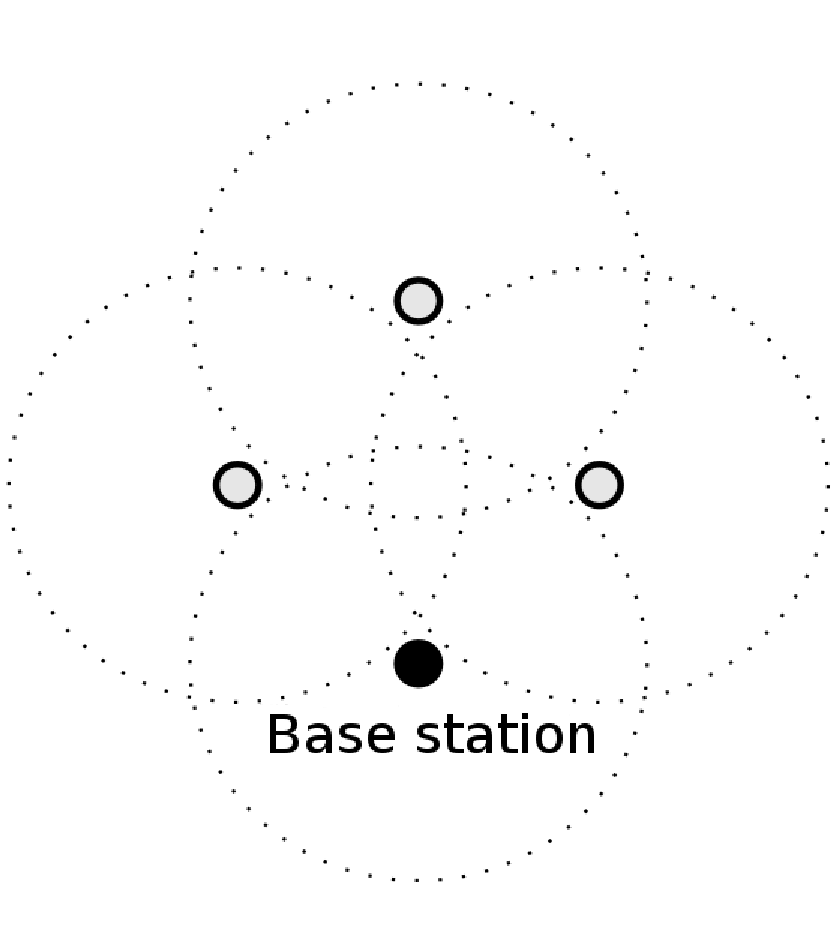
\includegraphics[scale=0.2]{fig/topology1} & 
%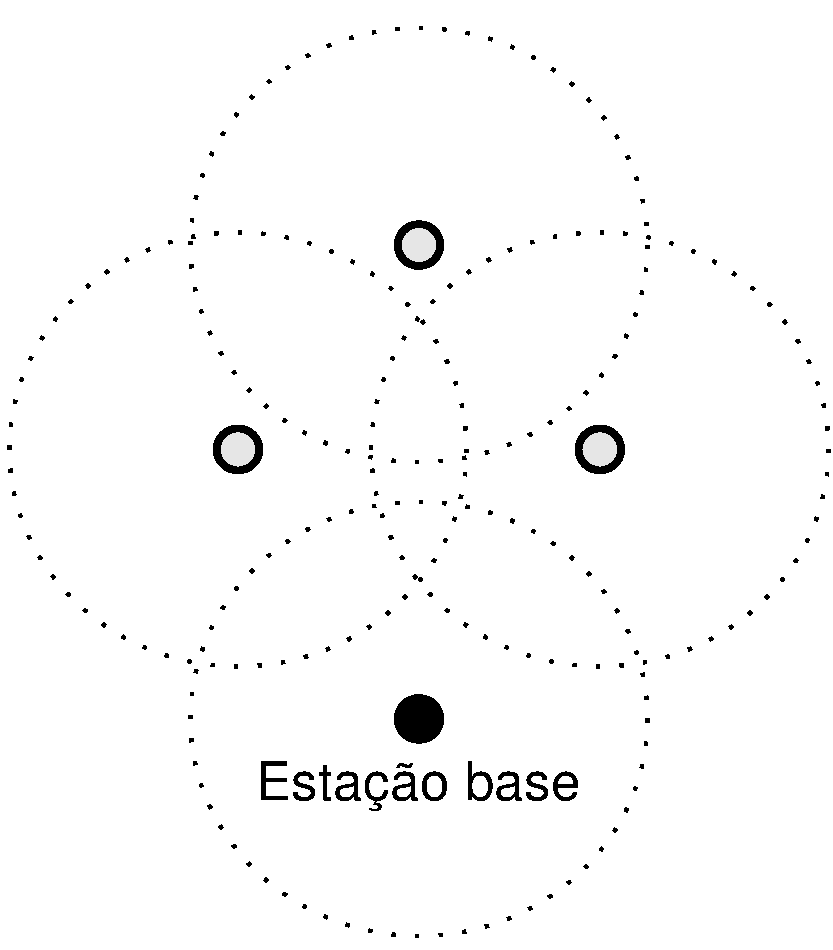
\includegraphics[scale=0.2]{fig/topology2} \\
%(a) & (b)
%\end{tabular}
%\caption{Topologies used to measure the protocol latency. (a) Base station has communication with all nodes (b) Base station does not have communication with all nodes.}
%\label{fig:topology}
%\end{figure}

%A Figura~\ref{fig:latency1} apresenta a média do tempo que a estação base leva para propagar os dados aos nodos a sua volta. Foi observado um desvio padrão de 0,0233 segundos. Este tempo não mudou alterando o número de receptores entre um e três, isto porque pacotes perdidos estão altamente correlacionados, ou seja, vários receptores perdem o mesmo conjunto de pacotes \cite{mnp}.
Figure~\ref{fig:latency1} shows the average time that the base station takes to propagate data to the nodes around it.
We observed a standard deviation of 0.0233 seconds.
This time did not change by changing the number of receivers between one and three.
This happens because loss packet is highly correlated, so multiple receivers lose the same set of packets~\cite{mnp}.

\fig{latency1}{Dissemination and reconfiguration time.}{scale=.57}

%A Figura~\ref{fig:latency2} mostra a média de tempo que os dados levam para serem propagados da estação base para nodos intermediários, e destes para o nodo fora de alcance da estação base (segunda topologia). É possível perceber que o tempo necessário para propagar dados entre nodos normais da rede é aproximadamente quatro vezes maior que o tempo gasto pela estação base, isto se deve ao fato que a estação base não executa a etapa de seleção de emissor, ou seja, não perde tempo divulgando sua versão e recebendo requisições para enfim se tornar um emissor e começar a disseminar os dados. O tempo de disseminação dos nodos intermediários apresentou um desvio padrão de 1,1288 segundos.
Figure~\ref{fig:latency2} shows the average time it takes to propagate the data from the base station to the intermediate nodes, and from these to the node out of range of the base station.
It is possible to notice that the time required to propagate data between normal network nodes is approximately four times greater than the time spent by the base station.
This is due to the fact that the base station does not perform the step of selecting a sender.
This way it wastes no time publishing its version and receiving requests to finally become a sender and begin to disseminate the data.
The time of intermediate nodes had a standard deviation of 1.1288 seconds.
 
\fig{latency2}{Dissemination time.}{scale=.57}

\subsection{Reconfiguration Time}
%Foi considerado como tempo de reconfiguração, o tempo que o nodo leva para atualizar sua memória de programa após ter recebido todos os dados necessários, via o protocolo de disseminação. Na estrutura proposta este tempo engloba: a chamada do \textsc{Reconfigurator}, os métodos \componente{p} e \componente{v} do semáforo, a chamada para o método \componente{Update}, a recuperação dos argumentos passados na mensagem ETP, a recuperação do objeto a ser atualizado em uma tabela hash, descobrir o endereço da \componente{vtable} e a escrita dos dados na flash. A Figura \ref{fig:latency1} mostra a média do tempo de reconfiguração obtido, sendo que o mesmo apresentou um desvio padrão de 0,0103 segundos.
The reconfiguration time encompasses the time a node takes to update its program memory after receiving all the necessary data.
In the proposed structure this time comprises: the call of \textsc{Reconfigurator}, methods \texttt{p} and \texttt{v} of the semaphore, the call to the \texttt{Update}, the recovery of arguments passed on the ETP message, the recovery of the object to be updated in a hash table, find the address of the \texttt{vtable}, and writing data in flash.
Figure~\ref{fig:latency1} shows the average reconfiguration time obtained. 
% It had a standard deviation of 0.0103 seconds. %%%%% isso ta errado

%Uma característica da arquitetura utilizada é que não é possível mudar apenas um byte por vez em sua memória flash. Esta memória só permite a escrita em páginas, cujo tamanho é de 256 bytes, e antes de reescrever uma página é necessário apagar seu conteúdo. Desta forma para atualizarmos uma parte da memória é necessário ler o conteúdo da página e armazená-lo em um buffer temporário, modificar apenas a parte desejada para enfim escrever na flash.
One feature of the Mica2 platform is that it is not possible to change only one byte at a time in its flash memory.
It allows only writing in pages (of 256 bytes), and before rewriting a page it is necessary to delete its contents.
Thus, in order to update a portion of memory, it is necessary to read the page content, store it in a temporary buffer, modify only the desired part of it, and finally write in the flash.

% Summary 

% Contributions: (1) common and simple interface (minor), (2)
% Power-management on embedded systems without using any complex
% high-cost methodology.
In this paper we presented an strategy to enable application-driven
power management in deeply embedded systems. In order to achieve this
goal we allowed application programmers to express when certain
components are not being used. This is expressed through a simple
power management interface which allows power mode switching of system
components, subsystems or the system as a whole, making all
combinations of components operating modes feasible. By using the
hierarchical architecture by which system components are organized in
our system, effective power management was achieved for deeply
embedded systems without the need for costly techniques or strategies,
thus incurring in no unnecessary processing or memory overheads.

A case study using a 8-bit microcontroller to monitor temperature in
an indoor ambient showed that almost 40\% of energy could be saved
when using this strategy. % and with minimal application intervention.

% Problems: concurrence. Describe the Thread problem.

% The paper also listed some identified problems on the path for
% power-aware software and hardware components, discussing and
% explaining how some of these problems have been solved in this work
% and how some of them can be solved, and will be, in future work.

% Even so, it still have its usability.




\bibliographystyle{abbrv}
\bibliography{references}

\balancecolumns
\end{document}